% GNUPLOT: LaTeX picture with Postscript
\documentclass{minimal}
% Set font size
\makeatletter
\def\@ptsize{7}
\InputIfFileExists{size17.clo}{}{%
   \GenericError{(gnuplot) \space\space\space\@spaces}{%
      Gnuplot Error: File `size17.clo' not found! Could not set font size%
   }{See the gnuplot documentation for explanation.%
   }{For using a font size a file `size<fontsize>.clo' has to exist.
        Falling back ^^Jto default fontsize 10pt.}%
  \def\@ptsize{0}
  \input{size10.clo}%
}%
\makeatother
\renewcommand*\mddefault{bx}%
% Load packages
\usepackage{graphicx}
\usepackage{color}
\makeatletter
% Select an appropriate default driver (from TeXLive graphics.cfg)
\begingroup
  \chardef\x=0 %
  % check pdfTeX
  \@ifundefined{pdfoutput}{}{%
    \ifcase\pdfoutput
    \else
      \chardef\x=1 %
    \fi
  }%
  % check VTeX
  \@ifundefined{OpMode}{}{%
    \chardef\x=2 %
  }%
\expandafter\endgroup
\ifcase\x
  % default case
  \PassOptionsToPackage{dvips}{geometry}
\or
  % pdfTeX is running in pdf mode
  \PassOptionsToPackage{pdftex}{geometry}
\else
  % VTeX is running
  \PassOptionsToPackage{vtex}{geometry}
\fi
\makeatother
% Set papersize
\usepackage[papersize={813.60bp,428.40bp},text={813.60bp,428.40bp}]{geometry}
% No page numbers and no paragraph indentation
\pagestyle{empty}
\setlength{\parindent}{0bp}%
% Load configuration file
\InputIfFileExists{gnuplot.cfg}{%
  \typeout{Using configuration file gnuplot.cfg}%
}{%
 \typeout{No configuration file gnuplot.cfg found.}%
}%
\usepackage{bm}
\begin{document}
\begingroup
  \makeatletter
  \providecommand\color[2][]{%
    \GenericError{(gnuplot) \space\space\space\@spaces}{%
      Package color not loaded in conjunction with
      terminal option `colourtext'%
    }{See the gnuplot documentation for explanation.%
    }{Either use 'blacktext' in gnuplot or load the package
      color.sty in LaTeX.}%
    \renewcommand\color[2][]{}%
  }%
  \providecommand\includegraphics[2][]{%
    \GenericError{(gnuplot) \space\space\space\@spaces}{%
      Package graphicx or graphics not loaded%
    }{See the gnuplot documentation for explanation.%
    }{The gnuplot epslatex terminal needs graphicx.sty or graphics.sty.}%
    \renewcommand\includegraphics[2][]{}%
  }%
  \providecommand\rotatebox[2]{#2}%
  \@ifundefined{ifGPcolor}{%
    \newif\ifGPcolor
    \GPcolortrue
  }{}%
  \@ifundefined{ifGPblacktext}{%
    \newif\ifGPblacktext
    \GPblacktexttrue
  }{}%
  % define a \g@addto@macro without @ in the name:
  \let\gplgaddtomacro\g@addto@macro
  % define empty templates for all commands taking text:
  \gdef\gplbacktext{}%
  \gdef\gplfronttext{}%
  \makeatother
  \ifGPblacktext
    % no textcolor at all
    \def\colorrgb#1{}%
    \def\colorgray#1{}%
  \else
    % gray or color?
    \ifGPcolor
      \def\colorrgb#1{\color[rgb]{#1}}%
      \def\colorgray#1{\color[gray]{#1}}%
      \expandafter\def\csname LTw\endcsname{\color{white}}%
      \expandafter\def\csname LTb\endcsname{\color{black}}%
      \expandafter\def\csname LTa\endcsname{\color{black}}%
      \expandafter\def\csname LT0\endcsname{\color[rgb]{1,0,0}}%
      \expandafter\def\csname LT1\endcsname{\color[rgb]{0,1,0}}%
      \expandafter\def\csname LT2\endcsname{\color[rgb]{0,0,1}}%
      \expandafter\def\csname LT3\endcsname{\color[rgb]{1,0,1}}%
      \expandafter\def\csname LT4\endcsname{\color[rgb]{0,1,1}}%
      \expandafter\def\csname LT5\endcsname{\color[rgb]{1,1,0}}%
      \expandafter\def\csname LT6\endcsname{\color[rgb]{0,0,0}}%
      \expandafter\def\csname LT7\endcsname{\color[rgb]{1,0.3,0}}%
      \expandafter\def\csname LT8\endcsname{\color[rgb]{0.5,0.5,0.5}}%
    \else
      % gray
      \def\colorrgb#1{\color{black}}%
      \def\colorgray#1{\color[gray]{#1}}%
      \expandafter\def\csname LTw\endcsname{\color{white}}%
      \expandafter\def\csname LTb\endcsname{\color{black}}%
      \expandafter\def\csname LTa\endcsname{\color{black}}%
      \expandafter\def\csname LT0\endcsname{\color{black}}%
      \expandafter\def\csname LT1\endcsname{\color{black}}%
      \expandafter\def\csname LT2\endcsname{\color{black}}%
      \expandafter\def\csname LT3\endcsname{\color{black}}%
      \expandafter\def\csname LT4\endcsname{\color{black}}%
      \expandafter\def\csname LT5\endcsname{\color{black}}%
      \expandafter\def\csname LT6\endcsname{\color{black}}%
      \expandafter\def\csname LT7\endcsname{\color{black}}%
      \expandafter\def\csname LT8\endcsname{\color{black}}%
    \fi
  \fi
  \setlength{\unitlength}{0.0500bp}%
  \begin{picture}(16272.00,8568.00)%
    \gplgaddtomacro\gplbacktext{%
      \csname LTb\endcsname%
      \put(1236,5125){\makebox(0,0)[r]{\strut{}$\bm{10^{-3}}$}}%
      \put(1236,5928){\makebox(0,0)[r]{\strut{}$\bm{10^{-2}}$}}%
      \put(1236,6731){\makebox(0,0)[r]{\strut{}$\bm{10^{-1}}$}}%
      \put(1236,7535){\makebox(0,0)[r]{\strut{}$\bm{10^{0}}$}}%
      \put(1236,8338){\makebox(0,0)[r]{\strut{}$\bm{10^{1}}$}}%
      \put(1379,4628){\makebox(0,0){\strut{}}}%
      \put(2403,4628){\makebox(0,0){\strut{}}}%
      \put(3427,4628){\makebox(0,0){\strut{}}}%
      \put(4450,4628){\makebox(0,0){\strut{}}}%
      \put(5474,4628){\makebox(0,0){\strut{}}}%
      \put(270,6695){\rotatebox{-270}{\makebox(0,0){\strut{}$\bm{n^{[1]}(p)}$ [fm$\bm{^3}$]}}}%
      \put(3743,4526){\makebox(0,0){\strut{}}}%
    }%
    \gplgaddtomacro\gplfronttext{%
      \csname LTb\endcsname%
      \put(4822,7986){\makebox(0,0)[r]{\strut{}$\bm{^{4}}$He LCA}}%
      \csname LTb\endcsname%
      \put(4822,7578){\makebox(0,0)[r]{\strut{}IPM}}%
      \csname LTb\endcsname%
      \put(4822,7170){\makebox(0,0)[r]{\strut{}central}}%
      \csname LTb\endcsname%
      \put(4822,6762){\makebox(0,0)[r]{\strut{}tensor}}%
    }%
    \gplgaddtomacro\gplbacktext{%
      \csname LTb\endcsname%
      \put(6275,5125){\makebox(0,0)[r]{\strut{}}}%
      \put(6275,5928){\makebox(0,0)[r]{\strut{}}}%
      \put(6275,6731){\makebox(0,0)[r]{\strut{}}}%
      \put(6275,7535){\makebox(0,0)[r]{\strut{}}}%
      \put(6275,8338){\makebox(0,0)[r]{\strut{}}}%
      \put(6418,4628){\makebox(0,0){\strut{}}}%
      \put(7442,4628){\makebox(0,0){\strut{}}}%
      \put(8466,4628){\makebox(0,0){\strut{}}}%
      \put(9490,4628){\makebox(0,0){\strut{}}}%
      \put(10514,4628){\makebox(0,0){\strut{}}}%
      \put(6669,6695){\rotatebox{-270}{\makebox(0,0){\strut{}}}}%
      \put(8783,4526){\makebox(0,0){\strut{}}}%
    }%
    \gplgaddtomacro\gplfronttext{%
      \csname LTb\endcsname%
      \put(9862,7986){\makebox(0,0)[r]{\strut{}$\bm{^{16}}$O LCA}}%
      \csname LTb\endcsname%
      \put(9862,7578){\makebox(0,0)[r]{\strut{}IPM}}%
      \csname LTb\endcsname%
      \put(9862,7170){\makebox(0,0)[r]{\strut{}central}}%
      \csname LTb\endcsname%
      \put(9862,6762){\makebox(0,0)[r]{\strut{}tensor}}%
    }%
    \gplgaddtomacro\gplbacktext{%
      \csname LTb\endcsname%
      \put(11316,5125){\makebox(0,0)[r]{\strut{}}}%
      \put(11316,5928){\makebox(0,0)[r]{\strut{}}}%
      \put(11316,6731){\makebox(0,0)[r]{\strut{}}}%
      \put(11316,7535){\makebox(0,0)[r]{\strut{}}}%
      \put(11316,8338){\makebox(0,0)[r]{\strut{}}}%
      \put(11459,4628){\makebox(0,0){\strut{}}}%
      \put(12483,4628){\makebox(0,0){\strut{}}}%
      \put(13507,4628){\makebox(0,0){\strut{}}}%
      \put(14530,4628){\makebox(0,0){\strut{}}}%
      \put(15554,4628){\makebox(0,0){\strut{}}}%
      \put(11710,6695){\rotatebox{-270}{\makebox(0,0){\strut{}}}}%
      \put(13823,4526){\makebox(0,0){\strut{}}}%
    }%
    \gplgaddtomacro\gplfronttext{%
      \csname LTb\endcsname%
      \put(14902,7986){\makebox(0,0)[r]{\strut{}$\bm{^{40}}$Ca LCA}}%
      \csname LTb\endcsname%
      \put(14902,7578){\makebox(0,0)[r]{\strut{}IPM}}%
      \csname LTb\endcsname%
      \put(14902,7170){\makebox(0,0)[r]{\strut{}central}}%
      \csname LTb\endcsname%
      \put(14902,6762){\makebox(0,0)[r]{\strut{}tensor}}%
    }%
    \gplgaddtomacro\gplbacktext{%
      \csname LTb\endcsname%
      \put(1236,1237){\makebox(0,0)[r]{\strut{}$\bm{10^{-3}}$}}%
      \put(1236,2040){\makebox(0,0)[r]{\strut{}$\bm{10^{-2}}$}}%
      \put(1236,2843){\makebox(0,0)[r]{\strut{}$\bm{10^{-1}}$}}%
      \put(1236,3647){\makebox(0,0)[r]{\strut{}$\bm{10^{0}}$}}%
      \put(1236,4450){\makebox(0,0)[r]{\strut{}$\bm{10^{1}}$}}%
      \put(1379,740){\makebox(0,0){\strut{}0}}%
      \put(2403,740){\makebox(0,0){\strut{}1}}%
      \put(3427,740){\makebox(0,0){\strut{}2}}%
      \put(4450,740){\makebox(0,0){\strut{}3}}%
      \put(5474,740){\makebox(0,0){\strut{}4}}%
      \put(270,2807){\rotatebox{-270}{\makebox(0,0){\strut{}$\bm{n^{[1]}(p)}$ [fm$\bm{^3}$]}}}%
      \put(3743,230){\makebox(0,0){\strut{}$\bm{p}$ [fm$\bm{^{-1}}$]}}%
    }%
    \gplgaddtomacro\gplfronttext{%
      \csname LTb\endcsname%
      \put(4822,4098){\makebox(0,0)[r]{\strut{}$\bm{^{48}}$Ca LCA}}%
      \csname LTb\endcsname%
      \put(4822,3690){\makebox(0,0)[r]{\strut{}IPM}}%
      \csname LTb\endcsname%
      \put(4822,3282){\makebox(0,0)[r]{\strut{}central}}%
      \csname LTb\endcsname%
      \put(4822,2874){\makebox(0,0)[r]{\strut{}tensor}}%
    }%
    \gplgaddtomacro\gplbacktext{%
      \csname LTb\endcsname%
      \put(6275,1237){\makebox(0,0)[r]{\strut{}}}%
      \put(6275,2040){\makebox(0,0)[r]{\strut{}}}%
      \put(6275,2843){\makebox(0,0)[r]{\strut{}}}%
      \put(6275,3647){\makebox(0,0)[r]{\strut{}}}%
      \put(6275,4450){\makebox(0,0)[r]{\strut{}}}%
      \put(6418,740){\makebox(0,0){\strut{}0}}%
      \put(7442,740){\makebox(0,0){\strut{}1}}%
      \put(8466,740){\makebox(0,0){\strut{}2}}%
      \put(9490,740){\makebox(0,0){\strut{}3}}%
      \put(10514,740){\makebox(0,0){\strut{}4}}%
      \put(6669,2807){\rotatebox{-270}{\makebox(0,0){\strut{}}}}%
      \put(8783,230){\makebox(0,0){\strut{}$\bm{p}$ [fm$\bm{^{-1}}$]}}%
    }%
    \gplgaddtomacro\gplfronttext{%
      \csname LTb\endcsname%
      \put(9862,4098){\makebox(0,0)[r]{\strut{}$\bm{^{56}}$Fe LCA}}%
      \csname LTb\endcsname%
      \put(9862,3690){\makebox(0,0)[r]{\strut{}IPM}}%
      \csname LTb\endcsname%
      \put(9862,3282){\makebox(0,0)[r]{\strut{}central}}%
      \csname LTb\endcsname%
      \put(9862,2874){\makebox(0,0)[r]{\strut{}tensor}}%
    }%
    \gplgaddtomacro\gplbacktext{%
      \csname LTb\endcsname%
      \put(11316,1237){\makebox(0,0)[r]{\strut{}}}%
      \put(11316,2040){\makebox(0,0)[r]{\strut{}}}%
      \put(11316,2843){\makebox(0,0)[r]{\strut{}}}%
      \put(11316,3647){\makebox(0,0)[r]{\strut{}}}%
      \put(11316,4450){\makebox(0,0)[r]{\strut{}}}%
      \put(11459,740){\makebox(0,0){\strut{}0}}%
      \put(12483,740){\makebox(0,0){\strut{}1}}%
      \put(13507,740){\makebox(0,0){\strut{}2}}%
      \put(14530,740){\makebox(0,0){\strut{}3}}%
      \put(15554,740){\makebox(0,0){\strut{}4}}%
      \put(11710,2807){\rotatebox{-270}{\makebox(0,0){\strut{}}}}%
      \put(13823,230){\makebox(0,0){\strut{}$\bm{p}$ [fm$\bm{^{-1}}$]}}%
    }%
    \gplgaddtomacro\gplfronttext{%
      \csname LTb\endcsname%
      \put(14902,4098){\makebox(0,0)[r]{\strut{}$\bm{^{108}}$Ag LCA}}%
      \csname LTb\endcsname%
      \put(14902,3690){\makebox(0,0)[r]{\strut{}IPM}}%
      \csname LTb\endcsname%
      \put(14902,3282){\makebox(0,0)[r]{\strut{}central}}%
      \csname LTb\endcsname%
      \put(14902,2874){\makebox(0,0)[r]{\strut{}tensor}}%
    }%
    \gplbacktext
    \put(0,0){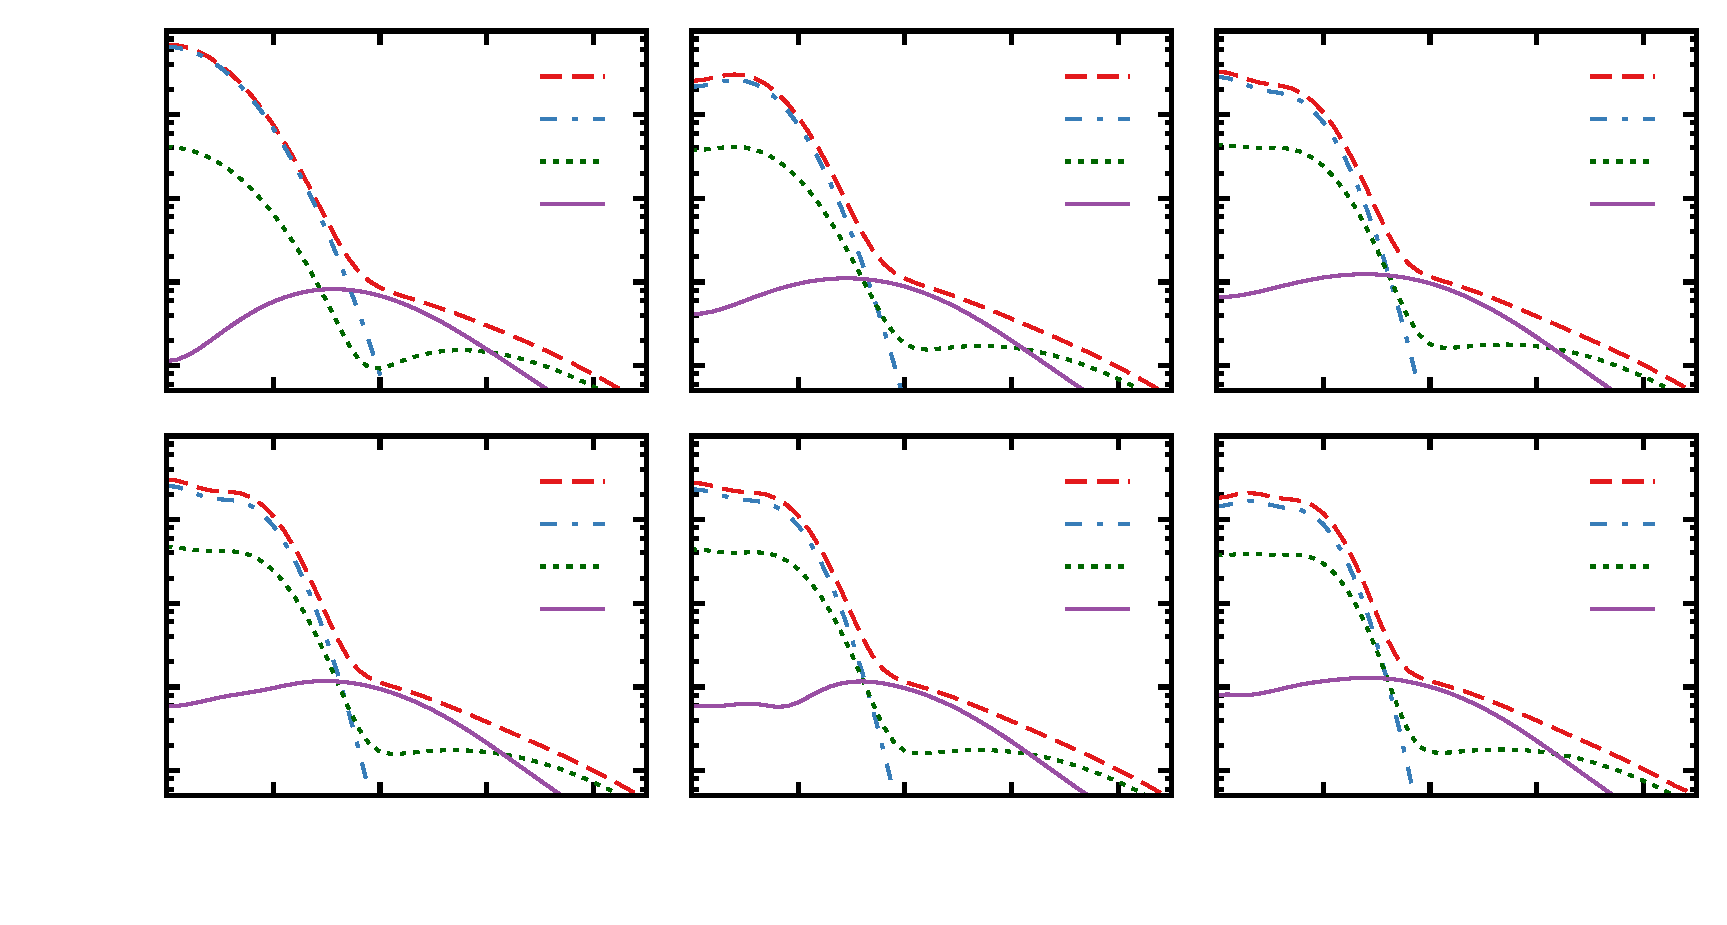
\includegraphics{dens_corr_ob-inc}}%
    \gplfronttext
  \end{picture}%
\endgroup
\end{document}
